\documentclass[dvipdfmx]{jarticle}
\pagestyle{empty}
\usepackage{tikz}
\usetikzlibrary{shapes,calc}
\begin{document}
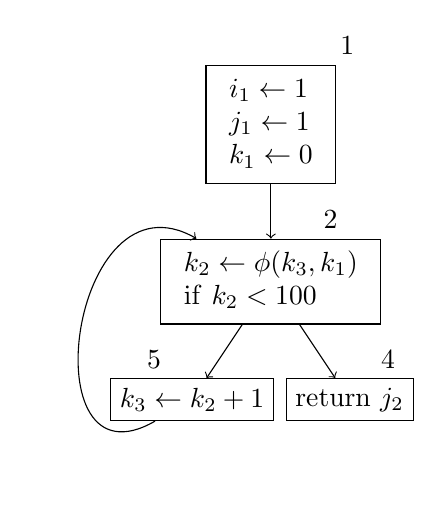
\begin{tikzpicture}
  \node[draw,label={45:$1$}] (B1) at (0,0) {
    $\begin{array}{l}
      i_1\leftarrow 1\\
      j_1\leftarrow 1\\
      k_1\leftarrow 0
  \end{array}$};
  \node[draw,label={45:$2$}] (B2) at (0,-2) {
    $\begin{array}{l}
%      j_2\leftarrow\phi(j_4,j_1)\\
      k_2\leftarrow\phi(k_3,k_1)\\
      \mathrm{if}\ k_2<100
    \end{array}$};
  % \node[draw,label={135:$3$}] (B3) at (-2,-4) {
  %   \mbox{\ \ \ \ \ }
  % };
  \node[draw,label={45:$4$}] (B4) at (1,-3.5) {
    $\mathrm{return}\ j_2$
  };
  \node[draw,label={135:$5$}] (B5) at (-1,-3.5) {
    $
%      j_3\leftarrow i_1\\
      k_3\leftarrow k_2+1
    $
  };
  % \node[draw,label={15:$6$}] (B6) at (1,-5.5) {
  %   $\begin{array}{l}
  %     j_5\leftarrow k_2\\
  %     k_5\leftarrow k_2+2
  %   \end{array}$
  % };
%   \node[draw,label={15:$7$}] (B7) at (0,-7.5) {
%     $\begin{array}{l}
% %      j_4\leftarrow\phi(j_3,j_5)\\
%       k_4\leftarrow\phi(k_3)
%     \end{array}$
%  };
  \path[->] (B1) edge (B2) (B2) edge (B4);
  \path[->] (B2) edge (B5);
  \path[->,out=210,in=150,looseness=2] (B5) edge (B2);
\end{tikzpicture}
\end{document}